%Chapter 7

% Chapter 7 from the standard thesis template
% Conclusions and Future work
\chapter{CONCLUSION AND FUTURE WORK} \label{ch:conclusion}

\section{Conclusion}
In this thesis we have shown that a SDR-based radiometer, using off the shelf components, is able to perform in a similar fashion to a traditional radiometer and may be used in the same applications. These applications may include soil moisture, ocean salinity and radio astronomy.   Using a SDR-based radiometer has several advantages over a traditional radiometer.  This includes the ability to filter an offending signals and may be a less expensive system by using commercial off the shelf components. The result is more widespread usage of radiometers that are able to use remote sensing to learn more about our planet and even the cosmos. Because a SDR-based radiometer offers high flexibility, changes to the system can be done very quickly and allows for implementations of other types of radiometers that is discussed in the next section.

\section{Future work}\label{Futurework}

The work in this thesis demonstrates an implementation of a SDR-based radiometer as a simple radiometer using software running on a personal computer.  Two possible future work items are: 1) Moving the signal processing to a FPGA or ASIC and 2) Building more complex radiometer systems such as a Dicke radiometer and correlating radiometer.  These topics will be covered in the following paragraphs.   

\emph{Removing the PC.}  For this thesis we focused on the software that would run on a PC or comparable computer system running a full operating system such as Linux.  This allows for rapid development by using software tools such as GNURadio to develop the SDR-based radiometer.  While this works for testing the theory on a SDR-based radiometer, it does require hardware that is capable of running a full operating system and the associated software.  Some radiometer applications would find this acceptable.  However, other remote sensing applications, such as space based applications, would require a more efficient configuration.  One solution is to move the signal processing from the PC to a FPGA or ASIC solution.  This will improve efficiency and weight by reducing the overhead of running the signal processing in an PC environment. 

\emph{Implementing different types of radiometers.}  
This thesis focused on a implementing a basic total power radiometer in software.  While this radiometer is effective, it relies on the fact that the components of the radiometer are stable.  Other types of radiometers have been developed that reduce the need to have a stable radiometer.  

%One of the largest challenges with a radiometer is improving the stability of the radiometer.  Drifts in temperature can greatly affect the gains from the LNAs and also change how much noise all components in the radiometer contribute.  A software defined radio can help as we are digitizing the signal as soon as possible.  This helps in eliminating the analog components for power detection and even for filtering, but does not eliminate all physical hardware, mainly the LNAs.  In this thesis, we did not focus on this issue since the tests were done in a controlled lab environment.

%However, a more compact, lower cost and easier setup would be to just have the LNAs attach directly to the SDR without any temperature compensation.  While this can be done, we have now lost stability in the LNAs and we need to compensate for that.  Several methods have been discussed to handle instability in a traditional radiometer.  Some of these methods would be suitable for implementation in a software defined radiometer.

A common method is a Dicke radiometer which was covered in this thesis.  A future work for our SDR-based radiometer would be to use a digitally generated noise source, such as a Gaussian noise source, and then switch between the antenna and this known noise source.  This noise source can also be adjusted and is performed in software, therefore stability in the noise source is not an issue.  

%One method that is discussed by William Goggins is to use a feedback loop to continuously adjust a variable attenuator [\cite{Goggins}].  In Goggins paper, he discusses using a servo that mechanically controls the attenuator.  However, since we are in the digital domain, we can control this all in software, and doing a feedback loop is quite easy for a computer to do.  

%Another method uses multiple temperature points that can be referenced at any time.  By using two known temperature references, we can quickly calibrate the radiometer[\cite{Hach}].  
 
Another method to improve stability and sensitivity is to correlate the information with another input which can be another antenna looking at the same source or can be two polarization from the same antenna[\cite{Clapp}].  This results in a two receiver system looking at the same source with two signal outputs, $S_1$ and $S_2$.  Since we are looking at the same source, both signals will be correlated in time, and when multiplied they will provide an output proportional to the strength of the source signal.  The noise introduced by each receiver will then have a lower correlation due to the random nature of the noise.  This results in a radiometer with a greater sensitivity due to the reduction of the noise even though two receivers are used [\cite{Fujimoto}].

{\begin{figure}[h!tb] 
\centering
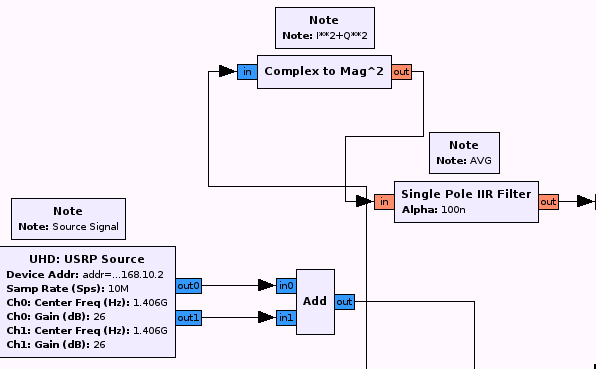
\includegraphics[width=14cm]{Images/N200_rad_corr.png}
\isucaption{A screenshot of an implementation of a correlating radiometer in GNURadio Companion.}
\label{correlating_sdr}
\end{figure}
}

The N200 software defined radio was chosen as it is capable of having two different daughter-cards plugged in.  Therefore, it is possible to have both sources enter the software defined radio and once digitized we can sum the magnitudes of the two incoming sources.  This is easy to do and is shown in Figure \ref{correlating_sdr}.

Although Figure \ref{correlating_sdr} shows a correlating SDR-based radiometer, it has not been tested.  In theory, this should correlate the signal and improve the sensitivity of the radiometer.  Additional experimentation will be required to confirm that this implementation operates as expected.

%Correlation also allows for unique ways for applications in radiometers including also performing beam steering [\cite{villarino02}]

%\subsection{Further testing}
%The improvements and additional features outlined in Section \ref{Futurework} will require additional testing and verification.  While it has been shown that a SDR-based radiometer operates identically to a traditional radiometer, further testing is needed to verify different operating modes of a software defined radiometer to their analog counterpart.

%\section{Closing statement}
%This thesis demonstrated that it is possible to use off the shelf components to create a SDR-based radiometer that can be used in any radiometer application that a traditional radiometer can be used in.  These applications may include soil moisture, ocean salinity and radio astronomy.  Use of a SDR-based radiometer can potentially allow radiometers to be used by a wider audience of users by creating an easy to user system and reducing the cost and hardware complexity that most radiometers require.  The result is more locations that are able to use radiometers as remote sensing tools to learn more about our planet and even the cosmos.
%----------------------------------------------------------
% End of Chapter 7.  Anything below this is extra information